\section{Methodology}
\label{sec:methodology}

We started from a lexical baseline based on Apache Lucene BM25 and progressively moved to a multi-stage neural pipeline.
Early experiments focused on analyzer choices, stopword lists and BM25 variants; these runs were useful to establish a stable baseline, but they also showed that lexical overlap alone is insufficient for this task.
\newline
We adopted a four-stage pipeline (Figure~\ref{fig:pipeline}) for the proposed information retrieval system, consisting of:
\begin{itemize}
    \item \textbf{Query Translation}: queries in French or German are first translated into English.
    \item \textbf{Query expansion}: we expanded the English query with additional context to bridge the gap between informal and domain specific language.
    \item \textbf{Retrieval}: we retrieved relevant documents from the corpus using the expanded query.
    \item \textbf{Reranking}: we reranked the retrieved documents based on their relevance to the original query.
\end{itemize}
For each of these stages, we experimented with different models, choosing the ones that performed better in relation to the others.

In the following sections all the four stages are precisely explained.

\begin{figure}[htbp]
    \centering
    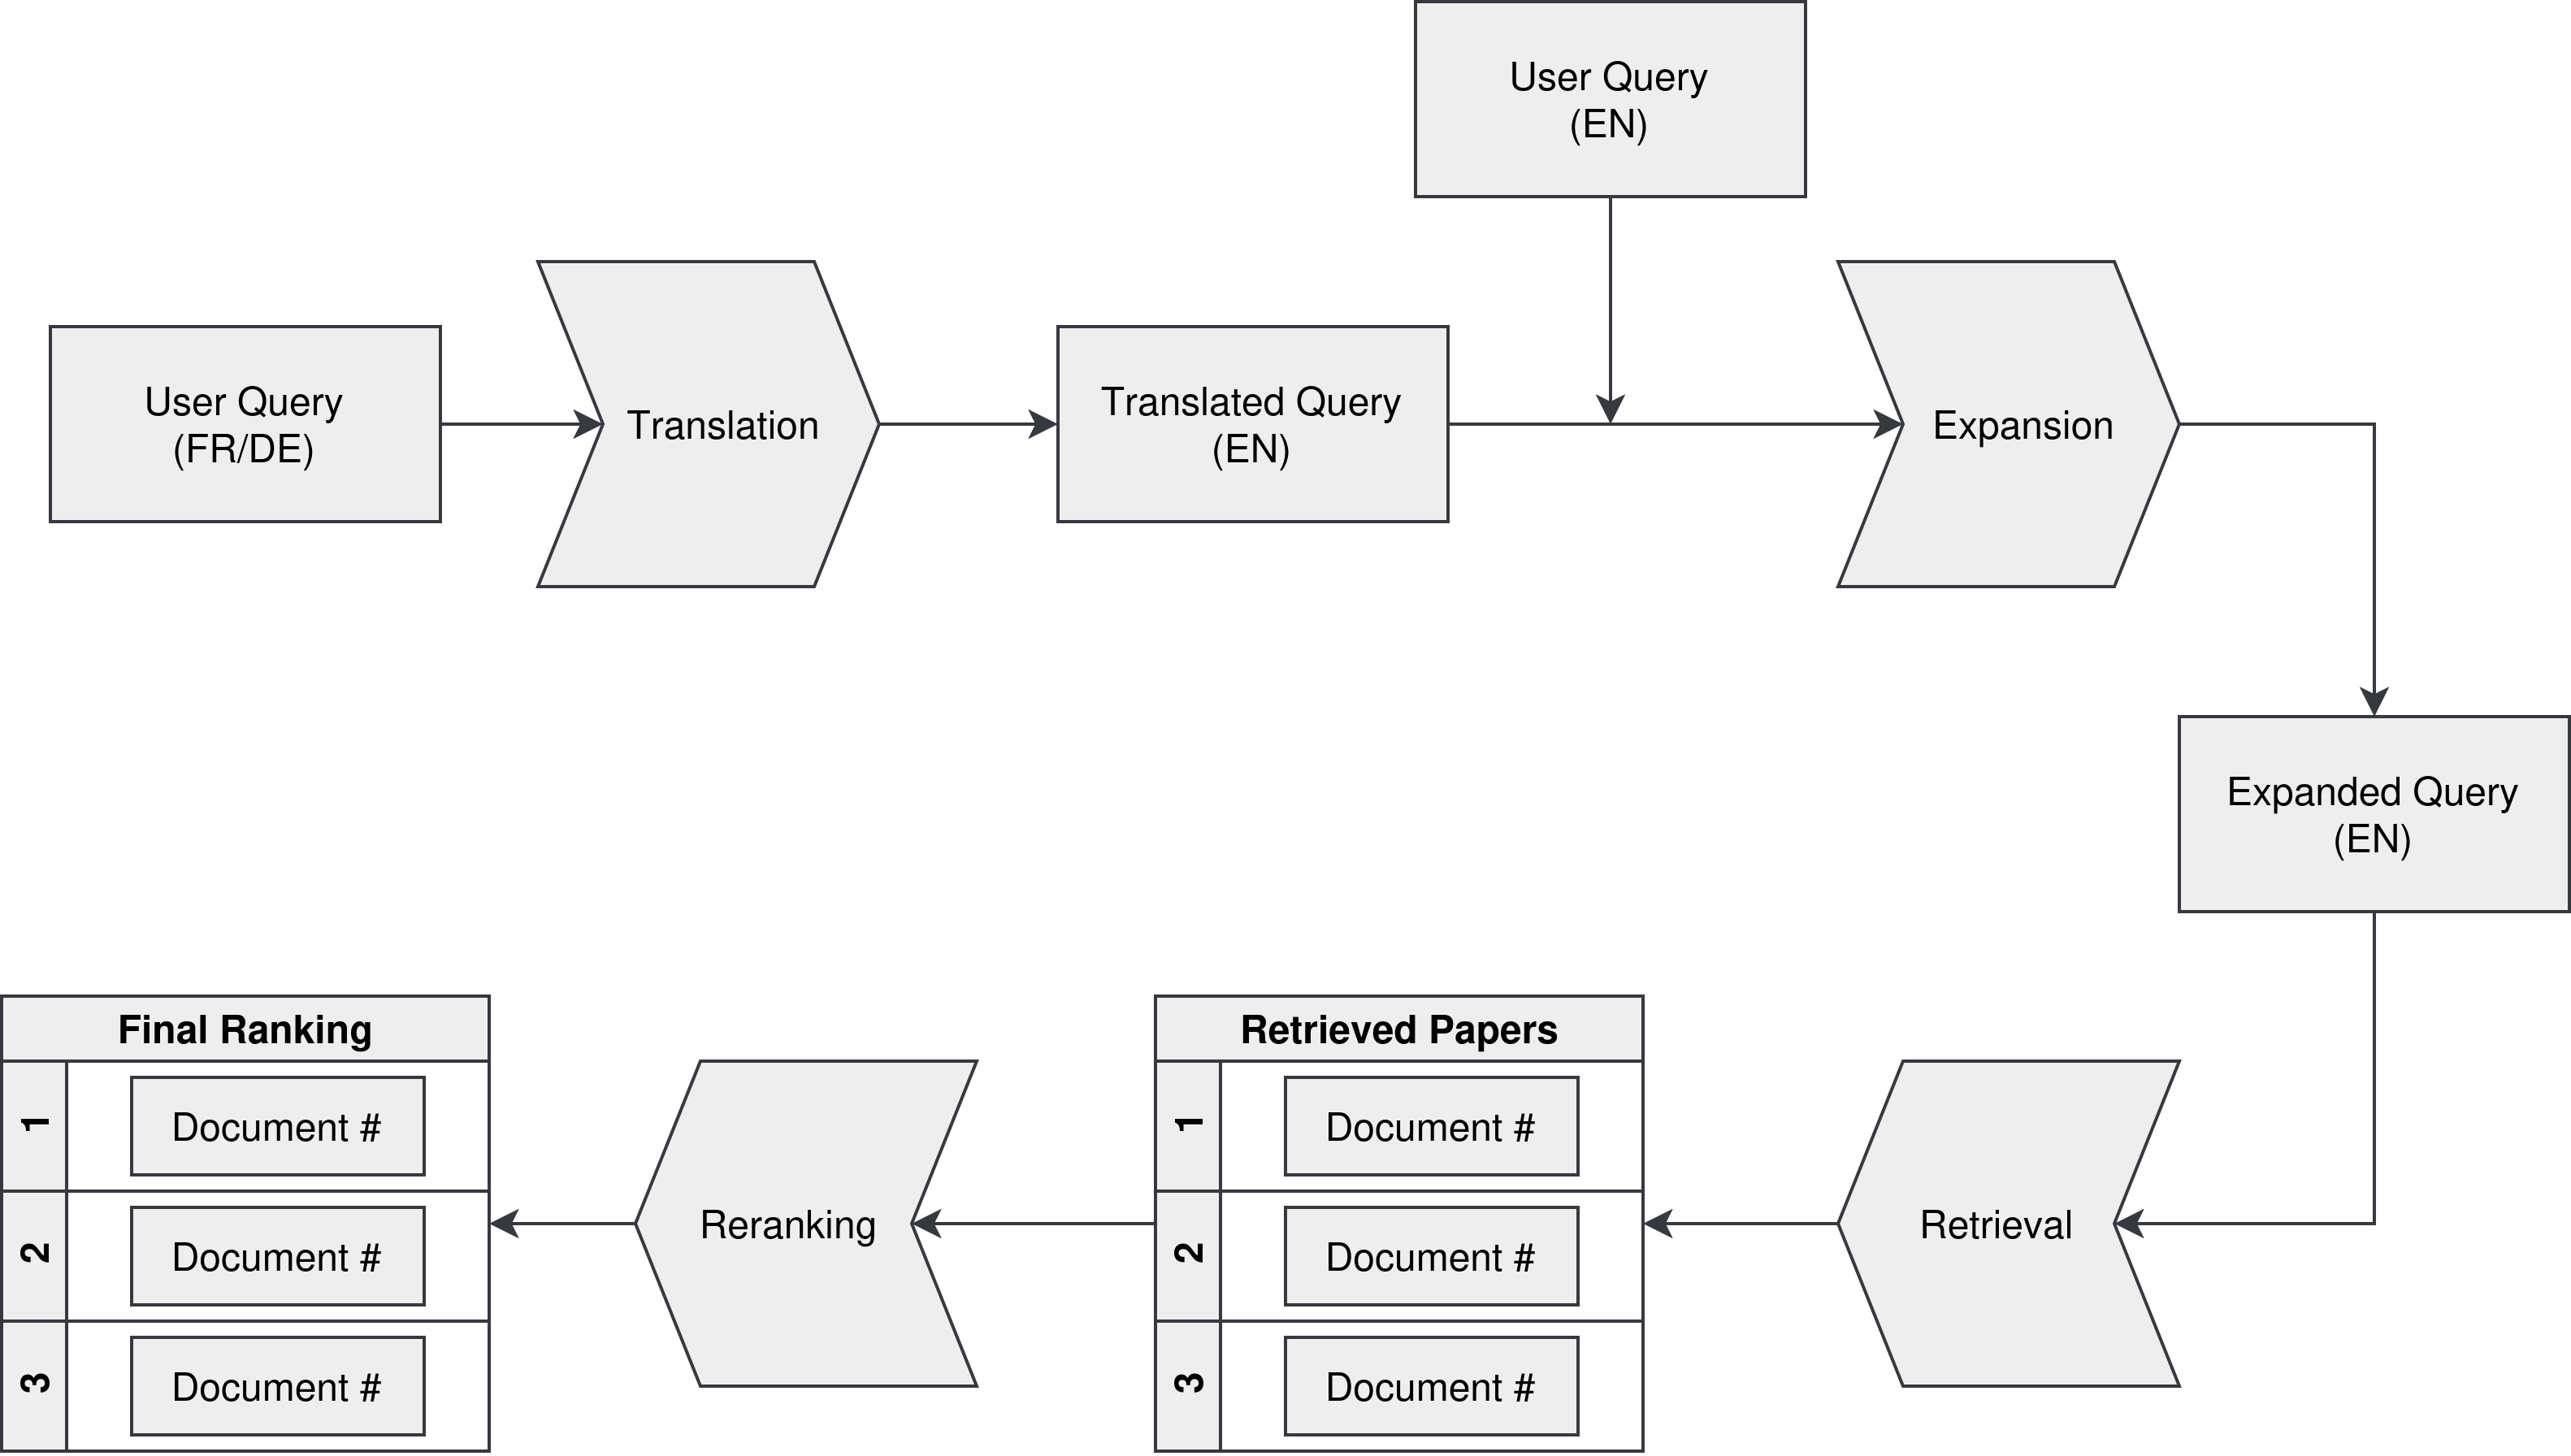
\includegraphics[width=0.8\linewidth]{figure/pipe.png}
    \caption{Four-stage pipeline for information retrieval.}
    \label{fig:pipeline}
\end{figure}

\subsection{Query translation} \label{sub:querytransl}
In the preliminary stage of out pipeline non-English queries (French and German) are translated into English. This is done query by query using the model \texttt{utter-project/EuroLLM-9B-Instruct-2512} with the following prompt:
\begin{promptbox}
\small
\ttfamily
\begin{flushleft}
\textit{system:} You are a professional translator.\\
Translate the user's text to English.\\
Output ONLY the English translation.\\
Do not include the original text, explanations, labels, or any other content.\\[0.8em]

\textit{user:} Translate this \{\textbf{French/German}\} text to English.\\
Output only the English translation, nothing else.\\[0.8em]

\{\textbf{Query original text $x$}\}
\end{flushleft}
\end{promptbox}
Given $x$ as the original query text, the model predict probabilities for the next token with \cite{huggingface_transformers_generation}: 
$$P(y_t=i\mid y_{<t},x)=\operatorname{softmax}(z_t/T)_i$$
Looking at our model configuration, the prediction becomes greedy, following \cite{utter_project_eurollm_9b_instruct_2512}: $$y_t=\arg\max_i P(y_t=i\mid y_{<t},x)$$
The resulting English queries are then fed into the following step of our pipeline. 

\subsection{Query Expansion} \label{sub:query-expansion}

Following the translation stage, each query is processed by a deterministic query-expansion module designed to reduce query–document vocabulary mismatch between short user claims and the terminology used in the scientific corpus. The module does not rely on generative LLM-based paraphrasing. Instead, it combines lexical feature extraction with dense semantic retrieval and neighborhood-based term induction. This design is consistent with the established role of query expansion in mitigating vocabulary mismatch in information retrieval and with the use of embedding models for semantic search.

\begin{itemize}
    \item The translated English query is first analyzed with spaCy’s \texttt{en\_core\_web\_sm} pipeline, which provides token-level linguistic annotations, including stop-word indicators and coarse-grained part-of-speech labels from the Universal POS tag set. Candidate lexical anchors are then identified by retaining tokens tagged as NOUN or PROPN while excluding stop words and tokens shorter than three characters. The resulting set is deduplicated to produce a compact lexical signature that captures the principal nominal content of the query. 
    
    \item The semantic expansion stage operates over a corpus in which each document is represented as the concatenation of its title and abstract. These title–abstract pairs are embedded with \texttt{BAAI/bge-large-en-v1.5}. In accordance with the documented BGE retrieval interface, query embeddings are produced by prepending the instruction \texttt{\{Represent this sentence for searching relevant passages:\}} to the translated query, whereas the corpus documents are encoded as retrieval targets. Similarity is then computed on normalized embeddings using the dot product. For unit-length vectors, dot-product scoring is equivalent to cosine similarity while being computationally more efficient. 
    $$s(q,d)=e_q^\top e_d=\sum_i e_{q,i}e_{d,i}$$
    Because embeddings \(e = \frac{v}{\lVert v\rVert_2}\) are L2-normalized \(e_q^\top e_d = \cos(q,d)\) \cite{bge_large_model_card}.\\
    The five highest-scoring documents are retained as the local semantic neighborhood used for expansion.

    In the described implementation, candidate expansion terms are extracted from the retrieved documents after lowercasing, ASCII normalization, mention and hashtag removal, stop-word filtering, and exclusion of short tokens. The candidate pool is aggregated across the retrieved neighborhood and assigned coarse weights derived from the semantic similarity of the source documents, so that terms originating from more similar neighbors contribute more strongly. Terms already present in the query are removed and the fifteen highest-ranking candidates are retained as explicit expansion terms.
    \[
K=\operatorname{unique}\{\ell(t): POS(t)\in\{\mathrm{NOUN},\mathrm{PROPN}\},\neg stop(t), |t|>2\}
\]
\[
w_h=\max(1,\operatorname{round}(5s_h))
\]
\[
c(t)=\sum_h w_h\,tf(t,d_h)
\]
\end{itemize}
The final expanded query is constructed by concatenating three components: the cleaned translated query, the noun and proper-noun-based keyword set extracted directly from the query and the expansion terms induced from the retrieved document neighbourhood.
This output expanded query is then used by the downstream retrieval pipeline.\\

Before confirming this as query expansion strategy, we have also tried to use two LLM models, \texttt{meta-llama/Llama-3.2-1B} and \texttt{openai/gpt-oss-20b} with the following prompt:
\begin{promptbox}
\small
\ttfamily
\begin{flushleft}
\textit{system:} ``Reasoning: \{reasoning\_effort\}''\\
You are a strict JSON-only retrieval query expansion generator.\\
Return the final answer only as valid JSON.\\[0.8em]

\textit{user:} You generate retrieval-specific query expansions.\\[0.5em]

Return only one valid JSON object with exactly these string fields:\\
\{\\
\hspace*{1em}``keywords'': ``\ldots'',\\
\hspace*{1em}``sparse'': ``\ldots'',\\
\hspace*{1em}``embedding'': ``\ldots'',\\
\hspace*{1em}``colbert'': ``\ldots'',\\
\hspace*{1em}``expanded'': ``\ldots''\\
\}\\[0.8em]

Rules:\\
-- Do not include markdown, code fences, emoji, commentary, arrays, or nested objects.\\
-- All five values must be strings.\\
-- Do not hallucinate facts.\\
-- Do not translate unless translation is already present in the query.\\
-- Preserve original-language terms.\\
-- \texttt{keywords}: compact important terms only; entities, nouns, technical terms, names, locations, dates, identifiers, acronyms, modifiers; no sentence.\\
-- \texttt{sparse}: lexical BM25/SPLADE-style expansion; exact-match terms, synonyms, acronyms, aliases, spelling and morphology variants; phrase fragments separated by spaces or semicolons; no long prose.\\
-- \texttt{embedding}: concise HyDE/query2doc-style natural-language semantic pseudo-document; include intent, context, and likely relevant-document framing.\\
-- \texttt{colbert}: concise late-interaction expansion; preserve important tokens and entities; add focused context and aliases; avoid synonym spam.\\
-- \texttt{expanded}: readable general-purpose merged expansion string combining the useful hints from the other fields.
\end{flushleft}
\end{promptbox}
This approach, which used a different expansion for each retrieval representation, did not improve performance. We therefore retained the simpler and more effective configuration based on a single expanded query. Section~\ref{sub:retrieval} describes in more detail how these expansion strategies were evaluated during retrieval.  
%Originally, we experimented with PRF-style expansion using semantic retrieval with \texttt{BAAI/bge-large-en-v1.5}.
% We then explored different methods for expansion,
% including Pseudo-Relevance Feedback (PRF) and similarity with static word embeddings using Word2Vec,
% testing these on both the original and the preliminary expanded queries.\newline

% In the final architecture, we used a multilingual LLM-based expansion script (\texttt{query\_expansion\_multilingual.py},
% default model \texttt{meta-llama/Llama-3.2-1B}) to generate multiple retrieval-oriented views of each query.
% The model is prompted to produce distinct representations,
% tailored to our multi-stage retrieval needs:
% \begin{itemize}
%     \item \textit{sparse}: A list of domain-specific keywords and technical synonyms (e.g., scientific nomenclature)
%     designed to maximize lexical overlap and mitigate the vocabulary mismatch in BM25-based retrieval.
%     \item \textit{dense}: A semantically enriched re-phrasing of the claim that provides a broader context, allowing the
%     bi-encoder in the next step of the architecture to produce more robust embeddings in the high-dimensional vector space.
%     \item \textit{ColBERT}: A structured, formal version of the claim (e.g., ``Serum levels and ICU admission'') that provides coherent
%     token sequences for fine-grained late-interaction scoring.
% \end{itemize}

% This multi-view expansion ensures that the downstream hybrid retriever can leverage both high-precision lexical matches
% and broad semantic overlaps. By generating these representations simultaneously within a single inference step of
% the same LLM,
% we maintain a coherent relationship between the different query ``views'', effectively providing a unified but multi-faceted
% context for the retrieval pipeline.\newline

% The resulting expanded queries are then fed into the multi-stage retrieval framework described next.

\subsection{Retrieval} \label{sub:retrieval}
The retrieval stage is designed as a high-recall candidate-generation step between query expansion and neural reranking. Its objective is not to make the final relevance decision but to ensure that the true source paper is included in a sufficiently large candidate set for the subsequent, more computationally expensive cross-encoder stage. For this reason, after experimenting with a Lucene BM25 baseline, BGE-M3 using dense vectors only and other bi-encoder models, the final pipeline adopts \textbf{BAAI/bge-m3} in a hybrid retrieval setting.

This choice reflects the nature of the task. Social media claims often contain informal paraphrases, hashtags, named entities, numerical values and fragments of scientific terminology. Therefore, relying exclusively on exact lexical overlap or exclusively on dense semantic similarity may discard useful evidence. Hybrid retrieval is better suited to this setting because it combines complementary retrieval signals and can offer higher accuracy and stronger generalization capabilities~\cite{bge-m3}.

The retriever searches the fixed paper collection provided by the task organizers. Each paper is represented at document level by concatenating its title and abstract and the retrieved unit is always the paper \texttt{pubkey}. We did not split papers into smaller chunks because the task requires identifying the source publication rather than retrieving a specific evidence passage. Using one representation per paper also avoids an additional chunk-to-document aggregation step. Although the collection includes metadata such as venue and authors, this hybrid retrieval stage uses only titles and abstracts to speed up the inference time.

All input queries are converted into plain English, either because they are originally written in English or because they are translated before retrieval, see Section~\ref{sub:querytransl}. They are then expanded using the procedure described in Sections~\ref{sub:query-expansion}.

We chose \textbf{BAAI/bge-m3} because it is well suited to this retrieval setting. The model can produce dense vectors, sparse lexical weights and ColBERT-style multi-vector representations from the same encoder.\\
This allows the retriever to combine broad semantic matching, exact term evidence and fine-grained token-level matching without switching between unrelated encoders.\\
For the dense representation, the document or query embedding is obtained from the normalized
CLS representation \cite{chen2024bgem3}:
\[
e=\operatorname{norm}(H[0])
\]
For the sparse representation, BGE-M3 assigns lexical weights to tokens \cite{bge_m3_docs}:
\[
w_{qt}=\operatorname{ReLU}(W_{lex}^\top H_q[i])
\]
The sparse similarity between a query and a paper is then computed over overlapping terms:
\[
s_{lex}=\sum_{t\in q\cap p} w_{qt}w_{pt}
\]

Candidate selection is performed in two steps. First, all documents are encoded as dense BGE-M3 vectors and searched with an inner-product FAISS index~\cite{faiss_documentation}. 
The dense FAISS score is computed using inner product \cite{faiss_metrics}:
\[
s_{IP}(q,d)=q^\top d
\]

Since the dense vectors are normalized, this inner product is equivalent to cosine similarity:
\[
q^\top d=\cos(q,d)
\]
This dense stage acts as an efficient broad filter over the whole collection. The default setting retrieves a large candidate pool of \texttt{candidate\_multiplier} $\times$ \texttt{top\_k}, with \texttt{candidate\_multiplier = 3} and \texttt{top\_k = 2000}, before the final truncation. 
The number of candidates passed to the hybrid rescoring stage is:
\[
K_c=\min(N,\max(K,Km))
\]

This deliberately large candidate set favours recall, which is more important than precision at this stage.

Second, the dense candidates are rescored using the sparse and ColBERT-style representations. The sparse component rewards important overlapping terms, while the ColBERT-style component captures local token correspondences that may be lost when each document is represented by a single dense vector~\cite{KhattabZaharia2020}.
The ColBERT-style late-interaction score is computed as \cite{khattab2020colbert}:
\[
s_{colbert}(q,d)=\frac{1}{N_q}\sum_{i=1}^{N_q}\max_{1\le j\le N_d} q_i^\top d_j
\]

The final configuration was selected through a series of development runs. We first tuned the lexical baseline by varying the Lucene analyzer, stop-word lists, stemming strategy and BM25 searcher variants. These experiments improved the classical baseline but also highlighted its limitations for this task: even with query expansion and reranking, BM25-based candidate generation remained more dependent on surface-level lexical overlap than desired.

We then evaluated dense retrieval with several bi-encoder models. Among these, \textbf{BAAI/bge-m3} achieved the strongest performance and improved the semantic coverage of the candidate set, particularly for paraphrased and multilingual claims. We also tested BGE-M3 in a hybrid retrieval setting, using a setup that differed slightly from the final configuration. In those experiments, sparse, dense, and ColBERT-style retrieval were performed using dedicated query expansions tailored to each retrieval mode. More specifically, each query was represented through three complementary views: an embedding view for semantic matching, a sparse view for lexical and term-based evidence, and a ColBERT view for fine-grained token-level interaction.

However, the best results in our analysis were obtained with a simpler configuration in which BGE-M3 hybrid retrieval used the same expanded query, described in the previous section, for all three retrieval modes. We then tested several weighting configurations. Among them, the run labelled \texttt{bge\_m3\_hybrid\_513} was retained because it provided the strongest recall-oriented trade-off among the retrievers evaluated without reranking. This configuration used weights of $0.5$, $0.15$ and $0.35$ for dense, sparse, and ColBERT scoring, respectively, with a multiplier of $3$ and a maximum hybrid input length of $384$.

A closely related configuration with a larger ColBERT weight achieved a nearly identical MRR@5 but a lower Recall@100. We therefore preferred the configuration that better matched the role of retrieval as a candidate generator. This choice was further confirmed by downstream experiments: reranking candidates from \texttt{bge\_m3\_hybrid\_513} consistently outperformed the corresponding BM25-based reranked runs. In addition, increasing the reranked candidate depth from a few hundred documents to between $1000$ and $2500$ documents permitted to increase the final recall by serving to the neural reranker a bigger candidate-pool to rerank.

We also experimented with a learned fusion strategy for the hybrid signals. In particular, the experimental setup included a LightGBM LambdaMART option that builds features from the dense, sparse, and ColBERT scores, together with normalized score variants and dense-rank features, and then learns how to combine them. However, the retained retrieval configuration uses simpler linear fusion, which is easier to reproduce and aligns well with the recall-oriented role of this stage.

The final hybrid retrieval score is therefore computed as:
\[
s(q, d) =
0.5\,s_{\text{dense}}(q, d)
+ 0.15\,s_{\text{sparse}}(q, d)
+ 0.35\,s_{\text{colbert}}(q, d).
\]

The largest weight is assigned to the dense score because it provides the main semantic signal. The sparse and ColBERT components add complementary lexical and fine-grained matching evidence. Candidates are sorted by this score in descending order and truncated to the final \texttt{top\_k}. The retrieval output is a JSON mapping from each query ID to an ordered list of paper \texttt{pubkeys}. Scores are not exported, because the next stage treats retrieval as a candidate generator and recomputes relevance using a cross-encoder over the returned document identifiers.


\subsection{Reranking} \label{sub:reranking}

The reranking stage receives the candidate list produced by the hybrid retriever and reorders it using cross-encoder models. Its goal is to improve early precision, especially MRR@5, while preserving as much recall as possible from the first stage.

\subsubsection*{Cross-encoder scoring}
Our strongest single-stage reranker is \texttt{nvidia/llama-nemotron-rerank-1b-v2}, a 1B-parameter LLaMA-based model fine-tuned as a sequence classifier. For each query-document pair, we build an input sequence using the official NVIDIA prompt template:
\begin{promptbox}
\small\ttfamily
question:\{query\} \textbackslash n \textbackslash n passage:\{passage\}
\end{promptbox}
The model computes a scalar logit $z \in \mathbb{R}$ through a linear classification head applied to the final hidden state, and the relevance score is obtained by applying a sigmoid:
\[
  s(q, d) = \sigma(z) = \frac{1}{1 + e^{-z}}
\]
Documents are then sorted in descending order of $s(q, d)$.
In practice, reranking deeper candidate pools (500--2500 documents) consistently produced better final results than shallower pools, confirming the importance of high recall at the retrieval stage to compensate for miss-labeling from weaker previous retrieval-stages. At this stage, queries are evaluated against the corpus of the documents taking into account their title, abstract and author.

We also evaluated alternative rerankers, including Qwen3 and GTE-ModernBERT variants

\subsection{Fine-tuning the Reranker} \label{sub:finetuning}
To improve the Nemotron reranker on the domain-specific characteristics of the CheckThat! task, we fine-tuned \texttt{nvidia/llama-nemotron-rerank-1b-v2} using Parameter-Efficient Fine-Tuning (PEFT) with Low-Rank Adaptation (LoRA)
on data from both the 2025 and 2026 editions of the task.

\subsubsection*{Training data and hard-negative mining}
Training examples are query-document pairs with binary labels: a positive document is the gold source paper associated with the query, while negative documents are hard negatives mined automatically using \texttt{sentence-transformers/static-retrieval-mrl-en-v1}. Hard negatives are selected from the range $[5, 50]$ nearest neighbors (by embedding similarity) that satisfy $\text{score} \leq 0.85$ and lie at least $0.05$ below the positive score in cosine similarity (absolute margin) preventing trivially easy or falsely relevant negatives from polluting training that would under-mine the effectiveness of the fine-tuning.

Training data combines two years of the task:
\begin{itemize}
  \item \textbf{2026 data}: split 90\% training / 10\% development. The development set is drawn exclusively from 2026 data for consistency with the official CT26 Task~1 evaluation protocol. Due to time-constraints we used just the en\_train datasets but we suppose that also German and French translated queries datasets could improve the quality of the fine-tuning;
  \item \textbf{2025 data}: all available topics (dev, test-gold, and train splits) are used entirely for training, never for development.
\end{itemize}
This design ensures that the dev set used to track MRR@5 during training is distribution-aligned with the contest test queries. Each training record contains one query, one positive passage and up to five hard negatives.

\subsubsection*{LoRA architecture}
To fine-tune the 1B-parameter base model with limited GPU memory, we apply LoRA~\cite{hu2022lora} with rank $r = 16$ and scaling factor $\alpha = 32$. Adapters are inserted into all attention and feed-forward projection layers:
\texttt{q\_proj}, \texttt{k\_proj}, \texttt{v\_proj}, \texttt{o\_proj}, \texttt{gate\_proj}, \texttt{up\_proj}, and \texttt{down\_proj}.
The classification head (\texttt{score}) is included in
\texttt{modules\_to\_save} and is fully updated during training. The task type is \texttt{SEQ\_CLS}, matching the sequence-classification objective of the reranker.

\subsubsection*{Training objective}
The model produces a single scalar logit $z$ per input pair.
Training minimizes binary cross-entropy with logits over all
positive ($y=1$) and negative ($y=0$) pairs in each batch:
\[
  \mathcal{L} = -\frac{1}{B}\sum_{i=1}^{B}
    \Bigl[ y_i \log \sigma(z_i) + (1 - y_i)\log(1 - \sigma(z_i)) \Bigr]
\]
where $B$ is the effective batch size and $\sigma$ is the sigmoid function. Gradient accumulation over 4 steps is used to simulate a larger effective batch size of 32 without additional memory overhead.

\subsubsection*{Optimization}
The model is trained with AdamW, a learning rate of $2 \times 10^{-5}$, a linear warmup over 10\% of the total training steps, and gradient clipping at norm 1.0. Training runs for 3 epochs with bfloat16 mixed precision and gradient checkpointing enabled to reduce VRAM usage. The checkpoint with the best MRR@5 on the 2026 development set is retained.

\subsubsection*{Inference}
At inference time, the LoRA adapter weights are merged into the base model via \texttt{merge\_and\_unload()} before scoring, so no PEFT overhead is incurred during evaluation. The scoring procedure and prompt format are identical to those of the base reranker (Section~\ref{sub:reranking}) and the fine-tuned model is used as a drop-in replacement in the reranking stage.

\subsection{Evaluation}
We evaluate systems on the CheckThat! Task 1 query sets by matching retrieved \texttt{pubkey}s against the gold \texttt{pubkey} for each query. The official optimization target is MRR@5, which we use as the primary score during model and parameter selection. In parallel, we track Recall@100 to monitor candidate-generation quality and to verify that reranking gains do not come from overly aggressive filtering.

For internal analysis, our evaluator also computes additional ranking metrics (e.g., Recall@1/5/10/100, Precision@1/5/10,
MAP, and nDCG@k). This broader view is useful to interpret trade-offs between recall-oriented retrieval settings and
precision-oriented reranking settings while keeping MRR@5 as the main criterion for reporting and model selection.
